\documentclass[9pt,twocolumn,twoside]{pnas-new}
\usepackage{gensymb}
\usepackage[colorinlistoftodos]{todonotes}

% new commands:
% q value
\newcommand{\qval}[1]{$q<10^{-#1}$}

% species names
\newcommand{\cel}{\emph{C.~elegans}}
\newcommand{\dicty}{\emph{D.~discoideum}}
\newcommand{\ecol}{\emph{E.~coli}}

% gene names
\newcommand{\gene}[1]{\emph{#1}}

\newcommand{\nlp}{\emph{nlp-31}}
\newcommand{\ftna}{\emph{ftn-1}}
\newcommand{\ftnb}{\emph{ftn-2}}
\newcommand{\egl}{\emph{egl-9}}
\newcommand{\cysl}{\emph{cysl-1}}
\newcommand{\nog}{\emph{nog-1}}
\newcommand{\rhy}{\emph{rhy-1}}
\newcommand{\vhl}{\emph{vhl-1}}
\newcommand{\eglvhl}{\emph{egl-9;vhl-1}}
\newcommand{\eglhif}{\emph{egl-9;hif-1}}
\newcommand{\hif}{\emph{hif-1}}
\newcommand{\fog}{\emph{fog-2}}
\newcommand{\nhr}{\emph{nhr-57}}
\newcommand{\lam}{\emph{lam-3}}

% protein names
\newcommand{\eglp}{EGL-9}
\newcommand{\rhyp}{RHY-1}
\newcommand{\nogp}{NOG-1}
\newcommand{\vhlp}{VHL-1}
\newcommand{\hifp}{HIF-1}
\newcommand{\fogp}{FOG-2}
\newcommand{\nhrp}{NHR-57}
\newcommand{\lamp}{LAM-3}
\newcommand{\cyslp}{CYSL-1}

% DE genes numbers:
\newcommand{\egln}{1,487}
\newcommand{\rhyn}{1,816}
\newcommand{\vhln}{605}
\newcommand{\eglvhln}{1,989}
\newcommand{\hifn}{481}
\newcommand{\eglhifn}{364}
\newcommand{\fogn}{1,896}
\newcommand{\total}{3,211}
\newcommand{\inall}{53}
\newcommand{\allup}{10}
\newcommand{\alldown}{13}

% downstream targets
\newcommand{\egltargets}{1}
\newcommand{\rhytargets}{0}
\newcommand{\vhltargets}{36}
\newcommand{\hiftargets}{120}
\newcommand{\hifohtargets}{27}

\templatetype{pnasresearcharticle}[9pt,twocolumn,twoside,lineno] % Choose template

\title{Genetic Analysis of a Metazoan Pathway using Transcriptomic Phenotypes}

% Use letters for affiliations, numbers to show equal authorship (if applicable)
% and to indicate the corresponding author
% \author[a,b]{David Angeles-Albores}
% \author[a,b]{Carmie Puckett Robinson}
% \author[a]{Brian Williams}
% \author[b]{Igor Antoshechkin}
% \author[a,b]{Paul W Sternberg}
%
% \affil[a]{Department of Biology and Biological Engineering, Caltech, Pasadena, USA, 91125}
% \affil[b]{Howard Hughes Medical Institute}
% \affil[*]{These authors contributed equally to this manuscript}

% Please give the surname of the lead author for the running footer
\leadauthor{Angeles-Albores}

% Please add here a significance statement to explain the relevance of your work
\significancestatement{
Measurements of global gene expression are often used as
descriptive tools capable of identifying genes that are downstream a
perturbation. In theory, there is no reason why measurements of global
transcriptomes could not be used as a quantitative phenotype for genetic
analysis in multicellular organisms. In fact, qPCR measurements of single or a
few reporter genes are already used to perform genetic network analysis. Here,
we show that transcriptomes can be used for epistasis analysis in a metazoan,
and that transcriptomes afford far more information per experiment than classic
genetic analysis. By using transcriptomes as quantitative phenotypes, we can
accurately predict interactions between genes, while at the same time
identifying genes common to a pathway.
When pathways branch, it is also possible to identify gene batteries that are
associated with each end of the branch point. Finally, genes that would result
in invisible visible phenotypes in an animal are not likely to be invisible at
the transcriptome phenotype due to the exquisite granularity present in these
structures, which represents an important advance towards studying small effect
genes that make up the majority of animals' genetic repertoire.
}

% Please include corresponding author, author contribution and author declaration information
\authorcontributions{
DA, CPR and PWS designed the experiments. CPR selected the
genes and extracted mRNA from all mutants. BW made the libraries. IA performed
all sequencing. DA developed the mathematical theory. DA wrote all computer code
and performed all analyses. DA made all the reporter strains and performed all
microscopy. DA, CPR and PWS wrote the manuscript.
}

\authordeclaration{The authors declare no conflict of interest.}
% \equalauthors{\textsuperscript{1}A.O.(Author One) and A.T. (Author Two)
% contributed equally to this work (remove if not applicable).}
\correspondingauthor{\textsuperscript{2}To whom correspondence should be
addressed. E-mail: pws@caltech.edu}

% Keywords are not mandatory, but authors are strongly encouraged to provide
\keywords{genetics $|$ RNA-Seq $|$ epistasis $|$ hypoxia $|$
          transcriptomics $ | $ systems biology}

\begin{abstract}
RNA-Seq is a technology that is commonly used to identify genetic modules that
are responsive to a perturbation. In theory, global gene expression could also
be used as a phenotype in complex metazoans, with all the implications that has
for genetic analysis. To that end, we sequenced the transcriptome of four single
mutants and two double mutants of the hypoxia pathway in \cel{}. We successfully
analyzed the single mutants in a blinded fashion to predict the genetic
relationships between the genes, and used the double mutants as a test of our
predictions and to infer the directionality of the relationship.
We show that genes along a pathway tend to decorrelate as a result of
alternative regulatory modes and crosstalk with other pathways; and that this
decorrelation accurately reflects functional distance between genes. As a
by-product of our analysis, we predict \hiftargets{} genes under the regulation
of \hif{}, and \vhltargets{} genes under the regulation of \vhl{}.
Transcriptomic perturbations suggest an important role of \hif{}-dependent
response in chromatin remodelling in \cel{}. Interactive graphics for this paper
can be found at \url{www.wormlabcaltech.github.io/mprsq}.
\end{abstract}

\dates{This manuscript was compiled on \today}
\doi{\url{www.pnas.org/cgi/doi/10.1073/pnas.XXXXXXXXXX}}

\begin{document}

% Optional adjustment to line up main text (after abstract) of first page with
% line numbers, when using both lineno and twocolumn options.
% You should only change this length when you've finalised the article contents.
\verticaladjustment{-2pt}

\maketitle
\thispagestyle{firststyle}
\ifthenelse{\boolean{shortarticle}}{\ifthenelse{\boolean{singlecolumn}}{\abscontentformatted}{\abscontent}}{}

% If your first paragraph (i.e. with the \dropcap) contains a
% list environment (quote, quotation, theorem, definition, enumerate, itemize...),
% the line after the list may have some extra indentation. If this is the case,
% add \parshape=0 to the end of the list environment.
\dropcap{G}enetic analysis of molecular pathways has traditionally been performed
through epistatic analysis. Epistasis occurs when two genes interact, either
directly (biochemical interaction of their gene products) or indirectly. If two
genes interact, and the mutants of these genes have a quantifiable phenotype,
the double mutant will have a phenotype that is not the sum of the phenotypes of
the single mutants that make up its genotype. Epistatic analysis remains a
cornerstone of genetics today~\cite{Phillips2008}.

Previous work in \emph{S. cerevisiae} and \dicty{} using microarrays has shown
that transcriptomes can be used to infer genetic relationships in simple
eukaryotes~\cite{Hughes2000, VanDriessche2005}. Additionally, eQTL studies in
\cel{} and \emph{Drosophila melanogaster} have established the usefulness of
transcriptomic phenotypes for population genetics studies~\cite{}.
\todo[inline]{Need citations.}
Developments in the area of transcriptomics have brought forward new protocols,
such as RNA-Seq~\cite{Mortazavi2008}, and have also made important progress
towards cheaper sequencing~\cite{Metzker2010}, better and faster abundance
quantification~\cite{Patro2014,Bray2016,Patro2015} and improved differential
analysis of gene expression~\cite{Pimentel2016,Trapnell2013}.
As a result, RNA-Seq has been successfully used to identify genetic %key regulatory
modules involved in a variety of processes, including T-cell
regulation~\cite{Singer2016,Shalek2013}, the \cel{} linker cell
migration~\cite{Schwarz2012}, or planarian stem cell
maintenance~\cite{VanWolfswinkel2014,Scimone2014}. For the most part,
the role of transcriptional profiling has been restricted to target gene
identification.
In cell culture, single-cell RNA-seq has seen significant progress towards using
transcriptomes as phenotypes with which to test genetic interactions
~\cite{Adamson2016,Dixit2016}.
More recently, we have shown the first identification of a developmental state
of \cel{} using whole-organism transcriptome profiling~\cite{Angeles-Albores2016a}.

To investigate the ability of transcriptomes to serve as quantitative phenotypes,
we selected mutants in the \cel{} hypoxia pathway for transcriptome sequencing.
% carmie:
Metazoans depend on the presence of oxygen in sufficient concentrations to
support aerobic metabolism. Genetic pathways evolved to rapidly respond to any
acute or chronic changes in oxygen levels at the cellular or organismal level.
These oxygen sensitive pathways are involved in a broad range of human
pathologies and they have been subject to investigation biochemical and
genetic approaches~\cite{Semenza2012}. These approaches identified the Hypoxia
Inducible Factors (HIFs) as an important group of oxygen responsive genes.

Hypoxia Inducible Factors are highly conserved in metazoans~\cite{Loenarz2011}.
A common mechanism for hypoxia-response induction is heterodimerization between a
HIF$\alpha$ and a HIF$\beta$ subunit. The heterodimer then initiates
transcription of target genes~\cite{Jiang1996}. The number and complexity of HIFs varies
throughout metazoans, with humans having three HIF$\alpha$ subunits and two
HIF$\beta$ subunits, whereas in the roundworm \emph{Caenorhabditis~elegans}
(\cel{}) there is a single HIF$\alpha$ gene, \hif{}~\cite{Jiang2001} and a single HIF$\beta$
gene, \emph{ahr-1}~\cite{Powell-Coffman1998}. HIF target genes have been implicated
in a wide variety of cellular and extracellular processes such as glycolysis,
extracellular matrix modification, autophagy and immunity~\cite{Semenza1994,
Bishop2004,Shen2005,Bellier2009,Semenza2012}.

Levels of HIF$\alpha$ proteins tend to be tightly regulated. Under conditions of
normoxia, \hifp{}$\alpha$ exists in the cytoplasm and partakes in a futile cycle
of continuous protein production and rapid degradation~\cite{Huang1996}.
\hifp{}$\alpha$ is hydroxylated by three proline hydroxylases
in humans (PHD1, PHD2 and PHD3) but is only hydroxylated by one proline
hydroxylase (\egl{}) in \cel{}~\cite{Kaelin2008}. \hifp{} hydroxylation increases its
binding affinity to Von Hippel Lindau Tumor Suppressor 1 (\vhlp{}), which allows
ubiquitination of \hifp{} leading to its subsequent degradation. In \cel{},
\eglp{} activity is inhibited by binding of \cyslp{}, and \cyslp{} activity is
in turn inhibited at the protein level by \rhyp{}, possibly by
post-translational modifications to \cyslp{}~\cite{Ma2012}.

% old:
% The hypoxia pathway is a conserved pathway that is found in all
% metazoans~\cite{Semenza2012}. It plays an important role in oxygen and iron
% homeostasis and in the immune response among
% others~\cite{Nizet2009,Ackerman2012,Kirienko2013}, and it is believed to play
% an important role in cancer appearance and progression, making it an attractive
% therapeutic target for disease~\cite{Semenza2003}.
% In \cel{} and other systems, \hifp{} is constitutively degraded by a futile
% cycle that involves hydroxylation by the EGLN1 ortholog
% \eglp{}~\cite{,Epstein2001,To2005}, followed by ubiquitination by the von
% Hippel-Lindau Suppressor 1, \vhlp{}~\cite{Bishop2004,Shao2009,Tanimoto2000,Jaakkola2001}.
% Inhibition of hydroxylation leads to accumulation of activated
% \hifp{}~\cite{Bishop2004}. Among the known targets of \hifp{} activation are
% \rhy{} and \egl{}. Increased \rhyp{} activates \eglp{}~\cite{Shen2006,Ma2012}.

Here, we show that transcriptomes contain strong, robust signals that can be
used to infer relationships between genes in complex metazoans by reconstructing
the hypoxia pathway in \cel{} using RNA-Seq.
Furthermore, we show that the phenomenon of phenotypic epistasis, a hallmark of
genetic interaction, holds at the molecular systems level.
We also demonstrate that transcriptomes contain sufficient information, under
certain circumstances, to order genes in a pathway using only single mutants.
Finally, we were able to identify genes that appear to be downstream of \egl{}
and \vhl{}, but are almost certainly not targets of \hif{}.
Using a single set of genome-wide measurements, we were able to observe and
quantitatively assess  significant fraction of the known transcriptional
effects of \hif{} in \cel{}.
A complete, interactive version of the analysis is also available at
\url{www.wormlabcaltech.github.io/mprsq}.

\section*{Results}
\subsection*{The hypoxia pathway controls thousands of genes in \cel{}}
\label{sub:summary}

We performed whole-organism RNA-seq of the hypoxia pathway at a moderate
sequencing depth (~7 million mapped reads for each individual replicate) under
normoxic conditions, which allowed us to measure 13,598 isoforms across all
replicates and genotypes, which constitutes over half of all isoforms in \cel{}.
In spite of the low sequencing depth, transcriptome profiling of the hypoxia
pathway revealed that this pathway controls thousands of genes in \cel{}. The
\egl{} transcriptome showed differential expression of \egln{} genes, similarly to
the \rhyn{} genes differentially expressed in \rhy{} mutants. The \vhl{}
transcriptome showed considerably fewer differentially expressed genes (\vhln{}),
possibly reflecting the known fact that it is a weaker controller of \hif{} than
\egl{}~\cite{Shao2009}. The \egl{};\vhl{} double mutant transcriptome showed
\eglvhln{} differentially expressed genes. The \hif{} mutant also showed a
transcriptomic phenotype involving \hifn{} genes. The \egl{};\hif{} double mutant
showed a similar number of genes with altered expression (\eglhifn{}).

\subsection*{Clustering visualizes epistatic relationships between genes}
\label{sub:Clustering}

As a first step in our analysis, we analyzed our data using a general
linear model (see~\ref{methods}) on logarithm-transformed
counts. Genes that are significantly altered between wild-type and a given
mutant have a genotype coefficient ($\beta$) that is statistically significantly
different from 0. We refer to these coefficients through the greek letter. These
coefficients are not identical to the average log-fold change per gene, although
they are loosely related to this quantity. Larger magnitudes of $\beta$
correspond to larger perturbations. These coefficients can be used to study the
RNA-Seq data in question.

Clustering is a well-known technique in bioinformatics that is used to identify
relationships between high dimensional data points~\cite{Yeung2003}. We wanted
to make sure that clustering by differential expression yielded genetically
relevant information. \hif{} exhibits no obvious phenotypes under normoxic
conditions, in contrast to \egl{}, which exhibits an egg-laying (\emph{egl})
phenotype in the same environment. \egl{}; \hif{} mutants suppress the
\emph{egl} phenotype. If transcriptomic phenotypes behave similarly to their
macroscopic counterparts, \hif{} should cluster with the \egl{}; \hif{} double
mutant, whereas \egl{} should cluster away from the \hif{} mutant.
Indeed, when blind, unsupervised clustering was performed on the data, three
clusters emerged. \hif{} and \egl{};\hif{} clustered together, indicating
suppression of the \egl{} phenotype; whereas \egl{}, \egl{};\vhl{}, \vhl{} and
\rhy{} all clustered separately. Finally, our negative control \fog{} was in its
own cluster (see Fig.~\ref{fig:dendrogram}). We conclude that expression data
contains enough signal to cluster genes in a meaningful manner in complex
metazoans.

% dendrogram
\begin{figure}%[tbhp]
\centering
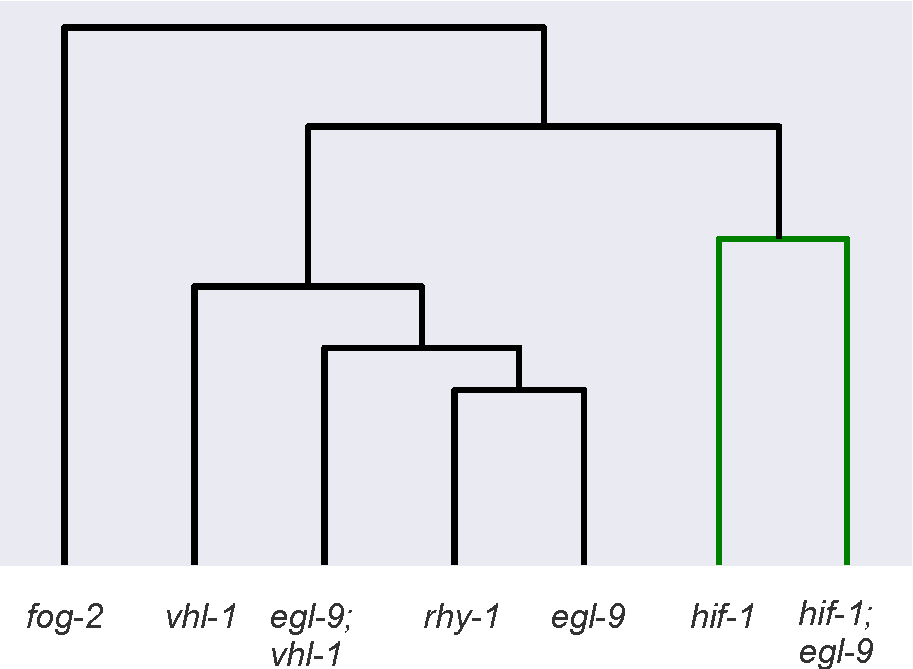
\includegraphics[width=0.75\linewidth]{figs/dendrogram.pdf}w
\caption{
Unsupervised aggregative clustering of various \cel{} mutants. Genes
cluster in a manner that is biologically intuitive. Genes that inhibit \hif{}
(i.e, \egl{}, \vhl{}, and \rhy{}) cluster far from \hif{}. \hif{} clusters with
the suppressed \egl{}; \hif{} double mutant. A a mutant \fog{} transcriptome,
used as an outgroup, clusters farthest away.
}
\label{fig:dendrogram}
\end{figure}

\subsection*{Reconstruction of the hypoxia pathway from first genetic principles}
\label{sec:reconstruct}
Having shown that the signal in the mutants we selected was strong enough to
cluster mutants using the regression coefficients, we set out to reconstruct the
hypoxia pathway from first genetic principles. In general, to reconstruct a pathway,
we must assess whether two genes act on the same phenotype (independence);
then we must measure whether these genes act additively or epistatically on the
measured phenotype; and if there is epistasis we must measure whether it is positive
or negative, in order to assess whether the epistatic regulation is a genetic
suppression or a synthetic interaction.

\subsubsection{Genes in the hypoxia mutant act on the same transcriptional phenotype}
\label{sec:phenotypes}
We observed that all the hypoxia mutants had significant overlap between their
differentially expressed transcriptomes relative to a wild-type control
(fraction of shared transcriptomes ranged from a minimum of 65 genes
shared between \hif{} and \egl{};\hif{} to a maximum of 1,249 shared genes between
\egl{} and \egl{};\vhl{}). For comparison, we also analyzed a previously published
\fog{} transcriptome~\cite{Angeles-Albores2016a}. \fog{} is involved in masculinization
of the \cel{} germline, which enables sperm formation, and has not been described
to be involved in the hypoxia pathway. The hypoxia pathway transcriptomes
and the \fog{} transcriptome showed similar overlap as the hypoxia pathway to itself
(123--618 genes). Given the similar overlaps between known interactors and an unknown
transcriptome, we conclude that the \fog{} mutant we studied acts on the same
phenotype as mutants from the hypoxia pathway.

% genetic correlations
\begin{figure}%[tbhp]
\centering
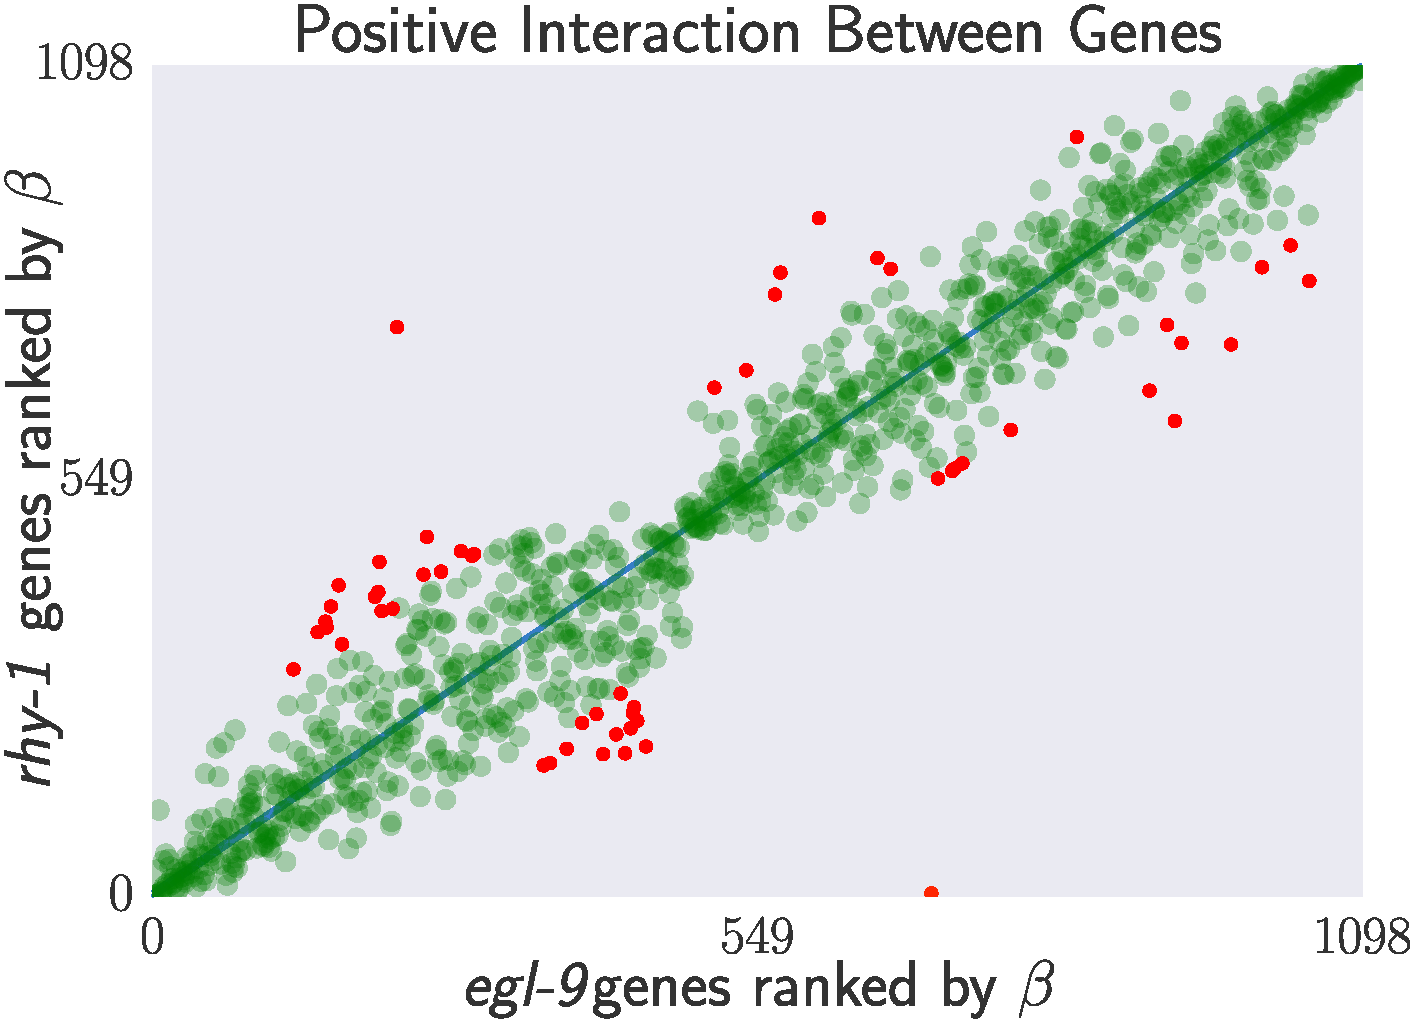
\includegraphics[width=\linewidth]{figs/correlative_genetics.pdf}
\caption{
Strong transcriptional correlations can be identified between genes
that share a positive regulatory connection. We took the \egl{} and the \rhy{}
transcriptomes, identified differentially expressed genes common to both
transcriptomes and ranked each gene according to its differential expression
coefficient $\beta$. We then plotted the rank of each gene in \rhy{} versus the
rank of the same gene in the \egl{} transcriptome. The result is an almost
perfect correlation. Green, transparent large points mark inliers to the
regression (blue line); red, opaque, small points mark outliers to the
regression. The two furthest outliers are annotated as pseudogenes in WormBase.
}
\label{fig:genetic_interactions}
\end{figure}

Although overlapping transcriptomes may be enough to conclude that a set of mutants
share a phenotype, we wanted to know whether we could draw out more information from
looking at quantitative agreement between perturbations. To this end, we rank-transformed
the regression coefficients $\beta$ for each transcriptome, and calculated lines
of best fit using Bayesian regression with a Student-T distribution to mitigate
noise from outliers (see Fig~\ref{fig:genetic_interactions}). For transcriptomes
associated with the hypoxia pathway, we found that these correlations tended to have
values as high as 0.98 with a tight distribution around the line of best fit,
whereas the correlations for mutants from the hypoxia pathway
with the \fog{} mutant were considerably weaker, with magnitudes between
0.6--0.85 and a considerably larger spread around the line of best fit.
Although \hif{} is known to be genetically repressed by \egl{}, \rhy{} and
\vhl{}~\cite{Epstein2001}, all the correlations
between these genes and \hif{} were negative. The overlap between
\hif{} and all other genes was small, and each overlap involved
different sets of genes, which suggests that we did not sequence deeply enough
to identify the nature of these positive interactions.
After we calculated the pairwise correlation between each transcriptome,
we weighted the result of each regression by the
number of differentially expressed isoforms shared by two transcriptomes and
divided by the total number of differentially expressed isoforms present in the
two transcriptomes, $N_\mathrm{overlap}/N_{\mathrm{g_1} \cup \mathrm{g2}}$.
The weighted regressions recapitulated a network with three `modules': A control
module, a responder module and an uncorrelated module (see Fig.~\ref{fig:heatmap}).
We were able to identify a strong positive interaction between \egl{} and \rhy{}.
The magnitude of this weighted correlation is derived from the fact that the
transcriptomes for these genes consisted of \egln{} and \rhyn{} significantly
altered genes respectively and the overlap between both genes was
extensive, which makes the weighting factor considerably larger than other pairs.
Likewise, the weak correlation between \hif{} and \egl{}, \vhl{} and \rhy{} is at
least partially the result of its relatively weak transcriptomic phenotype relative
to the other genes, particularly \egl{} and \rhy{}.
The fine-grained nature of transcriptional phenotypes means that these weighted
correlations between transcriptomes of single mutants are predictive of genetic
interaction.

% heatmap
\begin{figure}[tbhp]
\centering
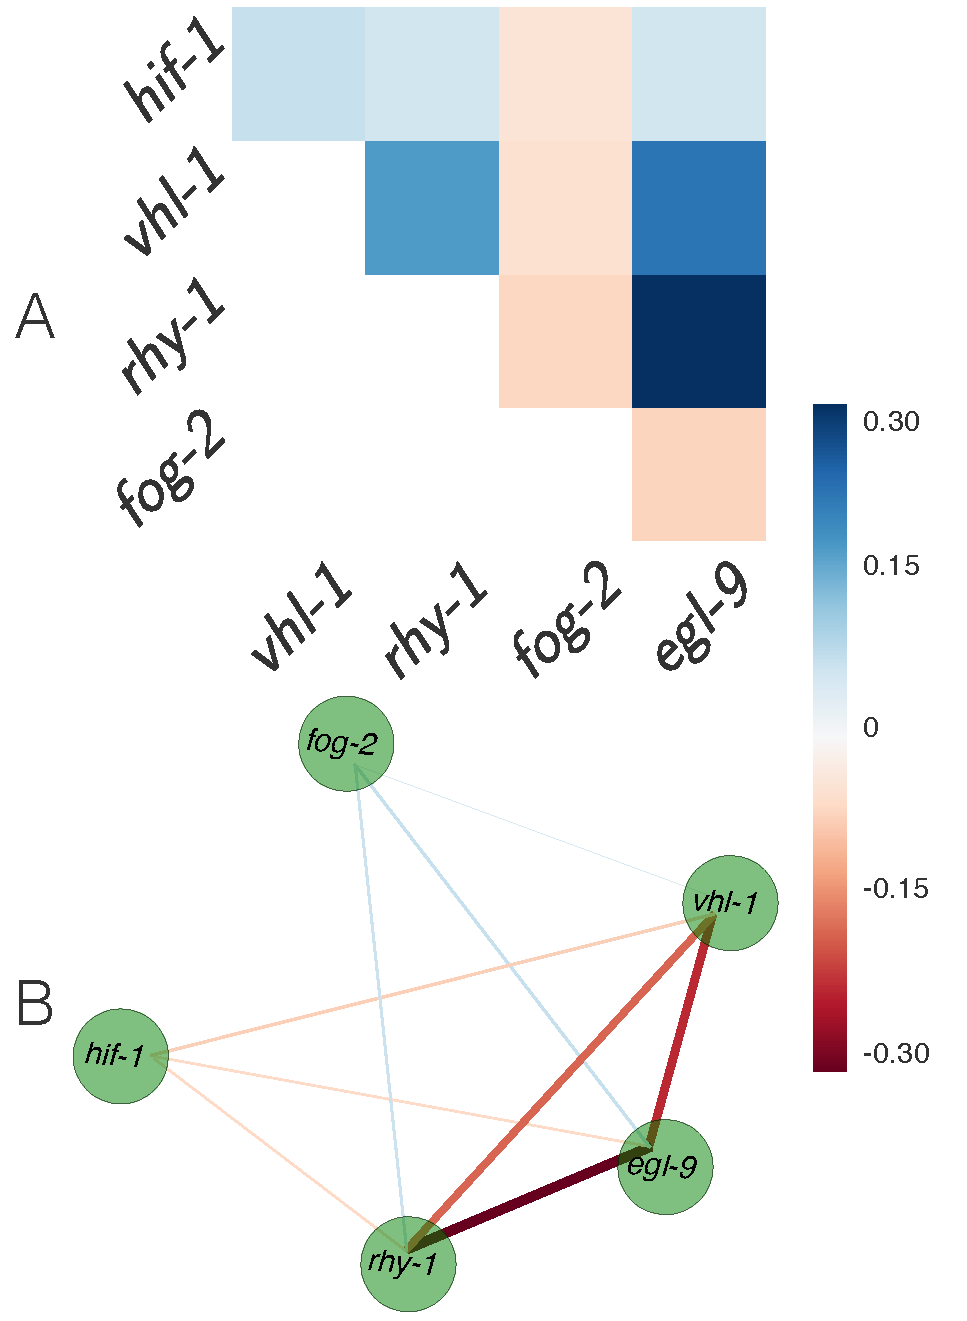
\includegraphics[width=\linewidth]{figs/bayesian_heat_map.pdf}
\caption{
\textbf{A}: Heatmap showing pairwise regression values between all
single mutants. \textbf{B}: Correlation network drawn from the diagram. Edge
width is proportional to the logarithm of the magnitude of the weighted
correlation between two nodes divided by absolute value of the weighted
correlation value of smallest magnitude. Edges are also colored according to the
heatmap in \textbf{A}.
}
\label{fig:heatmap}
\end{figure}

\subsubsection*{A quality check of the transcriptomic data reveals excellent agreement
            with the literature}
\label{sub:quality_check}
One way to establish whether genes are acting additively or epistatically to each
other is to perform qPCR of a reporter gene in the single and double mutants. This
approach was used to successfully map the relationships within the hypoxia
pathway (see, for example~\cite{Shao2009,Shen2006}). A commonly used reporter is
\nhr{}, which is known to exhibit large changes in expression upon induction of
\hifp{}\cite{Shen2006,Shen2005,Ackerman2012,
Park2012}. Likewise, \rhy{} and \egl{} are both known to be up-regulated
when \hifp{} becomes common in the cell~\cite{Powell-Coffman2010}.

Our dataset enables us to perform an equivalent computational experiment to qPCR
by selectively looking at expression of a few genes at a time. Therefore, we
queried the changes in expression of \rhy{}, \egl{}, \nhr{} and \lam{} as a negative
control. In our dataset, this gene be upregulated in \egl{}, \rhy{} and
\vhl{}, but remains unchanged in \hif{}.
The \egl{};\vhl{} had an expression level similar to \egl{}; whereas the
\egl{};\hif{} mutant showed suppression of the reporter expression. All of these
interactions reflect the literature.

% in silico qPCR
\begin{figure}[tbhp]
\centering
\includegraphics[width=\linewidth]{figs/qpcr.pdf}
\caption{
\textbf{Top}: \emph{In silico} qPCR.\@ We extracted
four genes (\rhy{}, \egl{}, \nhr{} and \lam{}, shown on the x-axis) and plotted
their regression coefficients, $\beta$, as measured for every genotype (represented by
one of six colors) to study the epistatic relationships between each gene.
Stars above a bar represent a regression coefficient statistically significantly
different from 0, meaning that expression is altered relative to a
wild-type control. Error bars show standard error of the mean value of $\beta$.
\nhr{} is an expression
reporter that has been used previously to identify \hif{}
regulators~\cite{Shen2006,Shao2009}. The \nhr{} mRNA levels replicate what is
observed in the literature. \lam{} is shown here as a negative control that
should not be altered by mutations in this pathway. The increases in the levels
of \egl{} and \rhy{} when repressors of \hif{} are knocked out are in agreement
with previous literature~\cite{Powell-Coffman2010}. We measured modest increases
in the levels of \rhy{} mRNA when \hif{} is knocked out. The mechanism behind
this is unclear. Negative and positive feedback loops from \hif{} into its
inhibiting genes could be a homeostatic mechanism.
}
\label{fig:qpcr}
\end{figure}

We also performed \emph{in silico} qPCR of every gene under scrutiny to get a
clearer idea of the relationships between them (see Fig.~\ref{fig:qpcr}). We
observed changes in \rhy{} expression consistent with previous
literature~\cite{Shen2006} when \hif{} is activated.
We also observed changes in \egl{}
expression when \egl{} was mutated. \egl{} is known as a hypoxia responsive
gene~\cite{Powell-Coffman2010} Although changes in \egl{} expression
were not statistically significant in \rhy{} and \vhl{} mutants, the mRNA levels
of \egl{} trended towards increased expression in these genotypes.
As with \nhr{}, the \egl{} and \rhy{} expression phenotypes were abrogated in
the \egl{};\hif{} mutant; whereas the \egl{};\vhl{} mutant showed expression
phenotypes identical to the \egl{} mutant.
Our dataset also shows that knockout of \hif{} resulted in a modest increase in
the levels of \rhy{}. This suggests that \hif{} is also a negative regulator of
\rhy{}, which constitutes a novel observation.
Taken together, these results indicate that RNA-seq data is at least equivalent
to qPCR for purposes of comparing gene expression of a reporter between genotypes.
Using a single reporter we would have been able to reconstruct an important fraction
of the genetic relationships between the genes in the hypoxia pathway.

\subsubsection*{Genes in the hypoxia pathway exhibit genome-wide epistasis}
As we have shown, it may be sufficient to extract the regression coefficients of a
previously known reporter gene and study just that pattern in order rebuild a
genetic pathway from RNA-seq data. However, we felt that by relying on a single
gene, or even a handful of genes to rebuild the pathway was throwing out all of
the valuable information present in our dataset. Therefore, we decided to
explore a new epistatic metric---genome-wide epistasis.

Ideally, any measurement of genome-wide epistasis should conform to certain
expectations. First, it should make use of the regression coefficients of as
many genes as possible. Second, it should be summarizable in a single,
well-defined number. Third, it should have an intuitive behavior, such that
the special values of the statistic (maximum, minimum, zero) should have an
unambiguous interpretation.

One way of defining genome-wide epistasis is to use linear regressions to describe
the relationship between the change in expression for a set of genes caused by a
single mutant and the change in expression in the same set of genes caused by a
double mutant containing the single mutant. The set of genes
to be studied can be defined as the set of differentially expressed genes common
to both genotypes.
Once the set is defined, the regression coefficient of each gene in the single
mutant can be plotted against the difference between the regression coefficients of
the double mutant and the single mutant. We reasoned that under ideal conditions,
such a plot would have an intuitive explanation. If two genes are acting
entirely independently of each other, the plot will show a line with slope equal
to 0. This is because is acting on entirely different sets of genes, so the
perturbation caused a gene $X^-$ is unchanged in the double mutant, $X^-Y^-$. If
two genes are acting only additively, then the plot will show a line with
slope $>0$ (and in fact, the slope should be equal to the slope between a plot of
the single mutants $X^-$ and $Y^-$). If two genes share a negative regulatory interaction,
then epistasis will be reflected in the plot as a line with a negative slope that
should approach $-1$, because
the double mutant, $X^-Y^-$ should have regression coefficients near 0, such that
the y-axis becomes equal to $-X^-$. If the two genes have a synthetic interaction,
we would expect that the slope must be positive and it must be greater than the
slope predicted by an additive model.

In our experiment, we studied two double mutants, \egl{};\hif{} and \egl{};\vhl{}.
We wanted to understand how well the global epistasis agreed with the literature
based on qPCR of single reporters. Therefore, we fit weighted linear regressions
to each of the four possible combinations (\egl{} vs. \egl{};\hif{};
\hif{} vs. \egl{};\hif{}; \egl{} vs. \egl{};\vhl{}; and \vhl{} vs. \egl{};\vhl{})
to measure the slopes of the lines of best fit.

We observe that the \egl{};\vhl{} mutant has an identical phenotype to the
\egl{} single mutant (slope = 0; see Table.~\ref{tab:double_mutant_comparison}).
On the other hand, \vhl{} has a positive slope, indicating that \egl{} is
additive to \vhl{}. However, this positive slope has to be less than the slope that
would be predicted by an additive model because the slope between \egl{};\vhl{} and
\egl{} is not statistically different from zero. Partial additivity indicates that
\egl{} inhibits \hif{} in \vhl{}-dependent and independent manners, which has
been documented in the literature~\cite{Shao2009}.

% double mutant analysis
\begin{table}%[tbhp]
{\centering
\caption{Response Modeling of Double Mutants to Single Mutants}
\begin{tabular}{llrrr}
Double Mutant & Single Mutant & $\Delta$ & SE & p-value\\
\midrule
1. \egl{};\vhl{} & \egl{} & $0.00$ & $0.01$ & $0.81$\\
2. \egl{};\vhl{} & \vhl{} & $0.28$ & $0.033$ & $10^{-15}$\\
3. \egl{};\hif{} & \egl{} & $-0.85$ & $0.074$ & $10^{-13}$\\
4. \egl{};\hif{} & \hif{} & $-0.18$ & $0.10$ & $0.10$\\
\bottomrule
\end{tabular}
\par
\label{tab:double_mutant_comparison}
}
\addtabletext{
Table showing changes between single and double mutants.
$\Delta$ is the result of a weighted-linear regression (WLS) between
$\beta_\mathrm{Single~Mutant}$ and $\Delta = \beta_\mathrm{Double~Mutant} -
\beta_\mathrm{Single~Mutant}$. $\Delta$ > 0 represents a more severe phenotype
than the single mutant. $\Delta$ < 0 represents a suppressed phenotype relative
to the single mutant. $\Delta$ = 0 is expected for linear pathways or genes that
are acting in linear or AND-gated fashion. $\Delta > 0$ is expected for genes
that are acting additively on a pathway. WLS were performed only on genes that
were significantly altered in both single mutants and the double mutant.
$1+\Delta$ is a very close approximation to the line of best fit between single
mutant and double mutant.
}
\end{table}

% epistasis graph
\begin{figure}[tbhp]
\centering
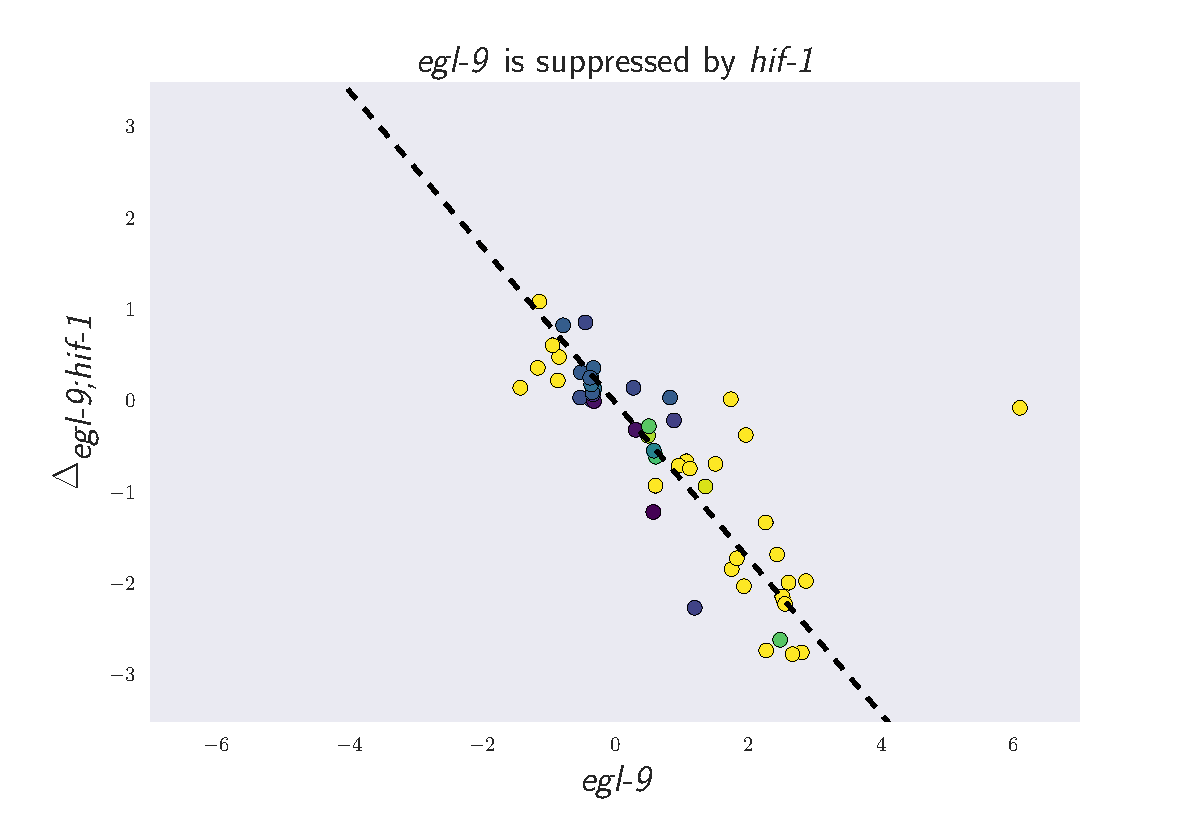
\includegraphics[width=\linewidth]{figs/egl9_epistatic_eglhif.pdf}
\caption{
The mutant \egl{} transcriptomic phenotype is suppressed by mutations in \hif{}.
The graph shows the $\beta$ coefficients for \egl{} in the x-axis, and the change
in $\beta$ coefficient between the \egl;\hif{} and \egl{} mutant. The dotted
line is the regression line between the complete \egl{} and \egl{};\hif{} shared
transcriptome. For clarity, only genes that were differentially expressed in the
\egl{}, \rhy{}, \vhl{}, \hif{} and \egl;\vhl{} datasets are shown. These points
constitute a very high-quality subset of the measured hypoxia response, as each
isoform was identified as differentially expressed in 5 independent genotypes.
The single outlier near (6, 0) is \nog{}. It is probably downstream of
\egl{}, and is not likely a \hif{} target.
}
\label{fig:egl9epistasis}
\end{figure}

On the other hand, comparison of the \egl{};\hif{} double mutant showed
suppression of the \egl{} transcriptomic phenotype. This suppression is expressed
in various ways. First, the double mutant shows less statistically significantly
differentially expressed genes than either single mutant. Secondly, the genes
that are common to the \egl{} and \egl{};\hif{} transcriptomes show decreased
expression in the \egl{};\hif{} mutant than they do in \egl{} on average (see
Fig.~\ref{fig:egl9epistasis}). The slope coefficient for the line of best fit is
$-0.85$. An interpretation for this slope value is that \hif{} suppresses
\emph{at least} 85\% of the \egl{} phenotype. Meanwhile, the genes that are common
to \hif{} and \egl{};\hif{} show no change in expression on average between
these two mutants, which shows that \egl{} and \hif{} are acting in the same pathway.

Because of the feedback between \hif{} and \egl{}, we expected a small subset of
genes to be differentially expressed in every hypoxia pathway mutant.
Therefore, we searched for genes that were differentially expressed in all our
hypoxia mutants (except the \hif{};\egl{} mutant because it has the least number
of differentially expressed genes), reasoning that these genes should constitute
an extremely high-quality picture of the hypoxia response, and should filter out other
pathways.
We identified \inall{} genes that satisfied these conditions, of which \allup{}
genes were up-regulated in every mutant, and \alldown{} genes were down-regulated.
These genes constitute a core response around the
circuit in question, and their behavior should reflect the genetic relationships
in our system the best. Although we performed the regressions using all the
overlapped genes between the single and double mutants, when we plotted only
these high-quality genes, we can see that they show beautiful agreement with the
global regressions (see \url{www.wormlabcaltech.github.io/mprsq} for all
interactive graphics).

\subsection*{Transcriptomic decorrelation can be used to infer functional distance}
\label{sub:decorrelation}

We were interested in figuring out whether RNA-Seq could be used to identify
functional interactions within a genetic pathway. Although there is no \emph{a
priori} reason why global gene expression should reflect functional interactions,
the strength of the unweighted correlations between genes in the hypoxia pathway
made us wonder how much information can be extracted from this dataset. Single
genes are often regulated by multiple independent sources. The connection between
two nodes can in theory be characterized by the strength of the edges connecting
them (the thickness of the edge); the fraction of sources that regulate both
nodes (the fraction of common inputs); and the fraction of genes that are
regulated by both nodes (the fraction of common outputs).
In other words we expected that expression profiles associated with a pathway
would respond quantitatively to quantitative changes in activity of the pathway.
Targeting a pathway at multiple points would lead to expression profile
divergence as we compare nodes that are separated by more degrees of freedom,
reflecting the flux in information between them.

% decorrelation
\begin{figure}[tbhp]
\centering
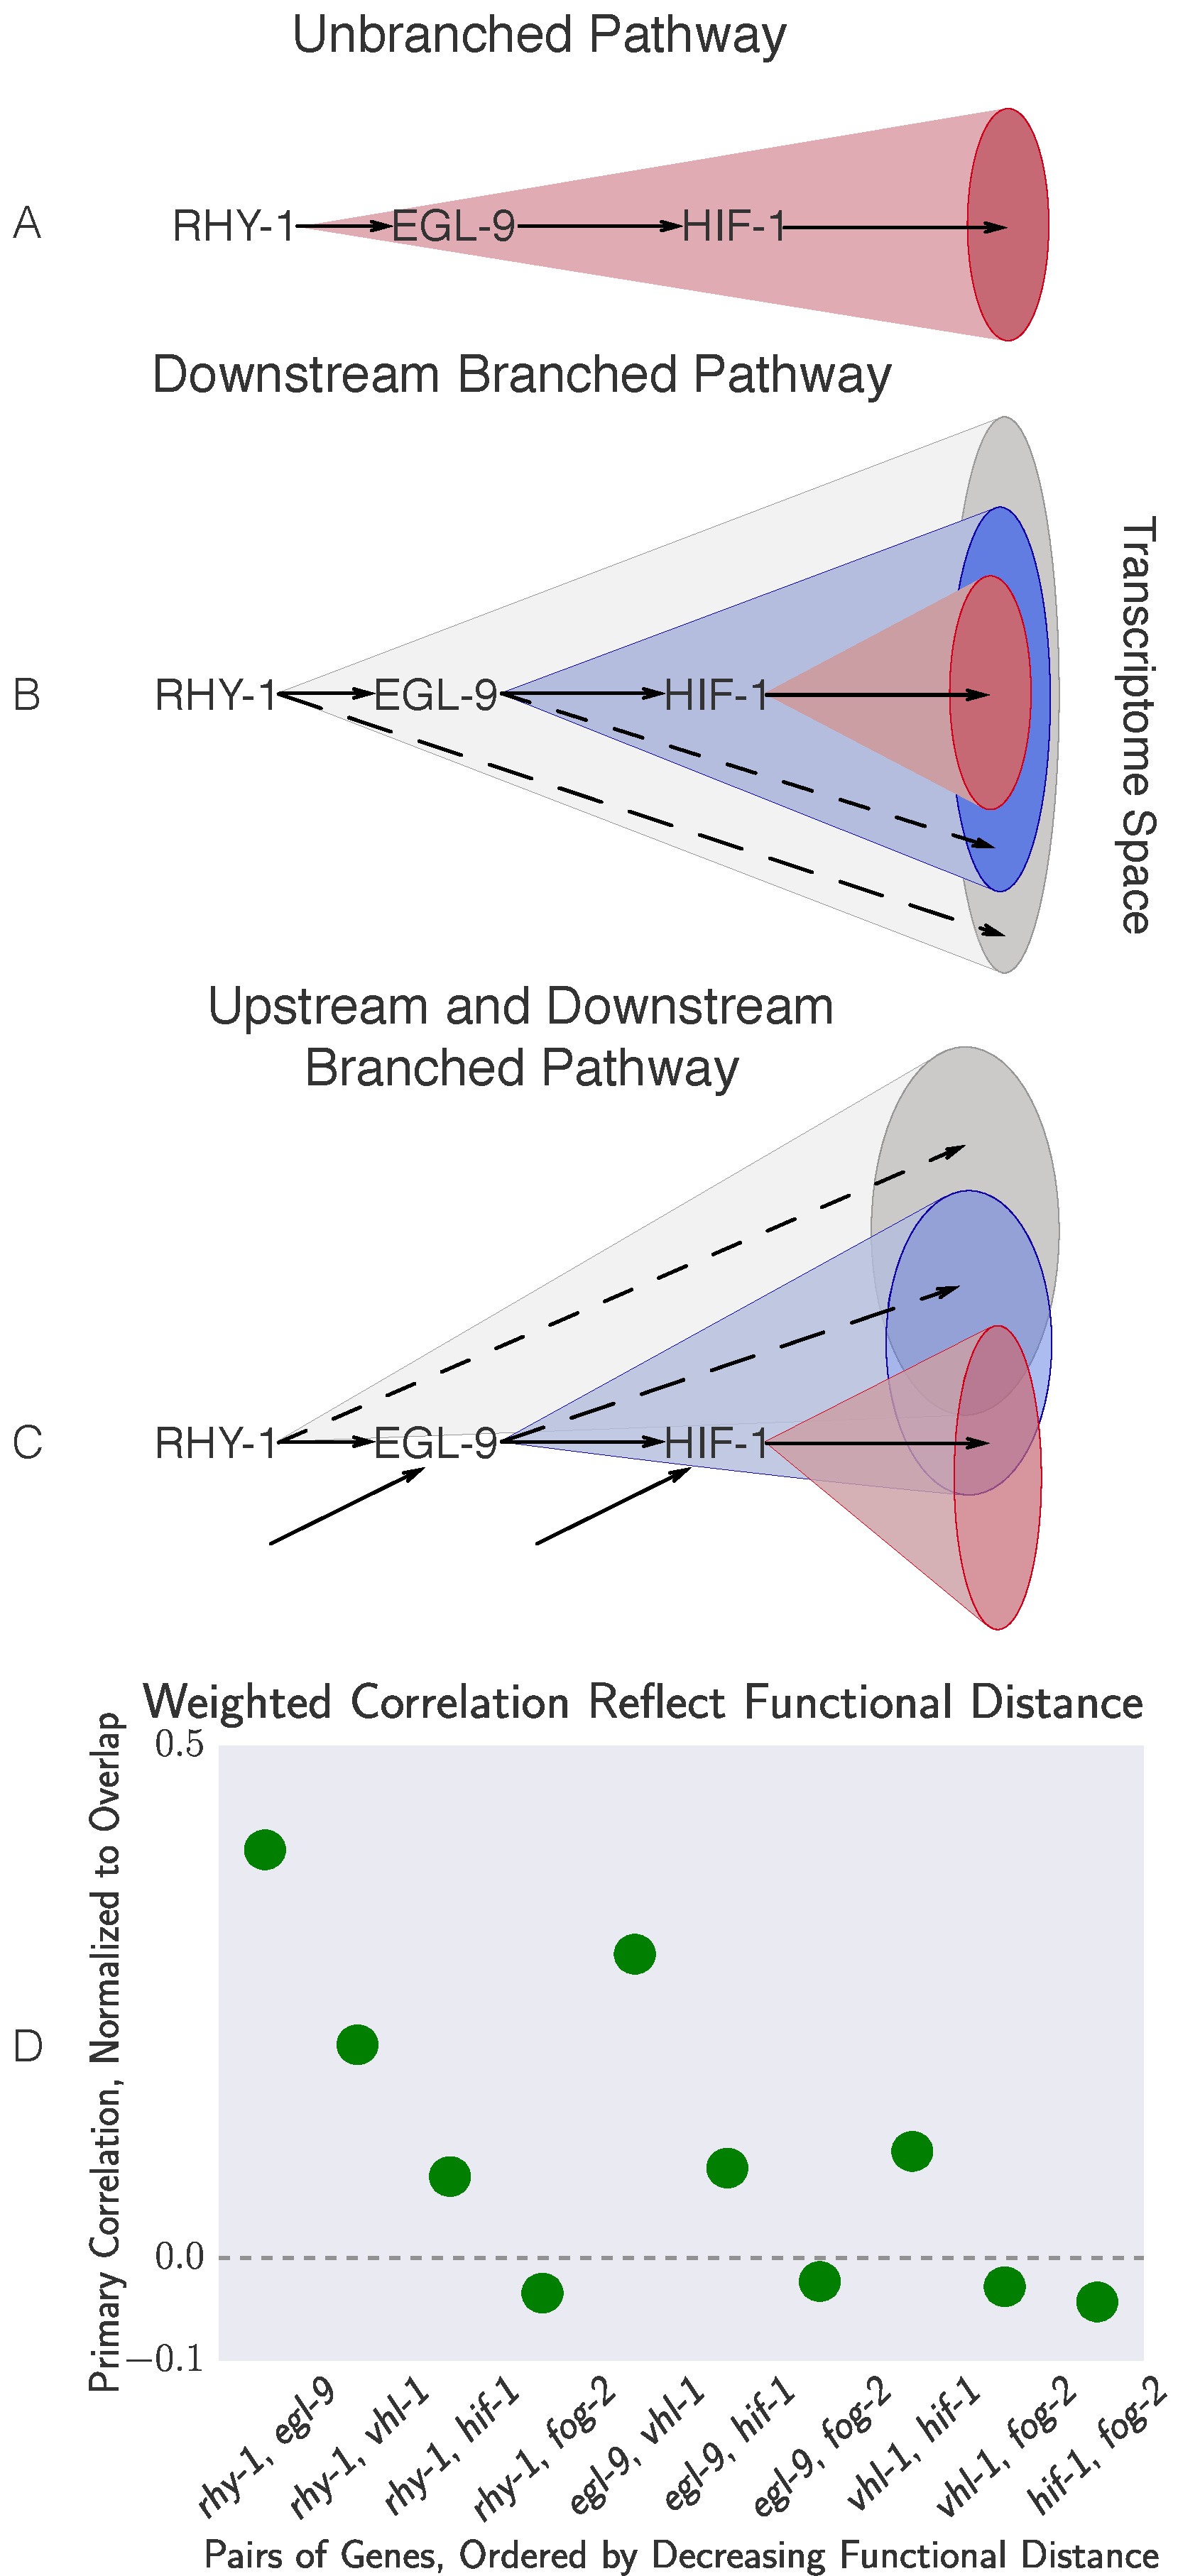
\includegraphics[width=\linewidth]{figs/decorrelation.pdf}
\caption{
Theoretically, transcriptomes can be used to order genes in a pathway under
certain assumptions. Arrows in the diagrams above are intended to show the
direction of flow, and do not indicate valence.
\textbf{A} A linear pathway in which \rhy{} is the only gene controlling \egl{},
which in turn controls \hif{} does not contain transcriptomes with enough
information to infer the order between genes.
\textbf{B} On the other hand, if \rhy{} and \egl{} have transcriptomic effects
that are separable from \hif{}, then the \rhy{} transcriptome should contain
contributions from \egl{}, \hif{} and \egl{}- and \hif{}-independent pathways.
This pathway contains enough information to infer order.
\textbf{C} If a pathway is branched in both upstream and downstream directions,
observed transcriptomes will show even faster decorrelation. Nodes that are
separated by many edges may begin to behave almost independently of each other
with marginal transcriptomic overlap or correlation, reflecting the weak control
distant nodes exert on each other.
\textbf{D} The hypoxia pathway can be ordered according to functional distance.
The rapid decay in correlation is probably due to a mixture of upstream and
downstream branching that happens along this pathway.
}
\label{fig:decorrelation}
\end{figure}

We investigated the possibility that transcriptomic signals do in fact contain
relevant information about the degrees of separation by weighting the robust
bayesian regression of each pair of genes by
$N_\mathrm{Intersection}/N_{\mathrm{Union}}$. We plotted the weighted
correlation of each gene pair, ordered by increasing functional distance
(see Fig.~\ref{fig:decorrelation}). In every case, we see that the weighted
correlation decreases monotonically due mainly, but not exclusively, to
decreasing $N_\mathrm{Overlap}$.
We believe that this result is not due to random noise or insufficiently deep
sequencing. Instead, we propose a framework in which every gene is regulated
by multiple different molecular species, which induces progressive decorrelation.
This decorrelation in turn has two consequences. First, decorrelation within a
pathway implies that two nodes may be almost independent of each other if the
functional distance between them is large. Second, it may be possible to use
decorrelation dynamics to infer gene order in a pathway, as we have done with
the hypoxia
pathway\footnote{
An important question is whether a looped circuit
like the hypoxia pathway can be ordered in the way we have ordered it in
Fig.~\ref{fig:decorrelation} since a loop does not technically have a beginning.
One explanation is that we studied the hypoxia pathway under normoxic conditions,
and therefore the control of \hif{} over \rhy{} and \egl{} is weak, effectively
turning the looped pathway into a linear one. Probably, under hypoxic conditions
the pathway would effectively be reversed.
}.

\subsection*{The circuit topology of the hypoxia pathway explains patterns in
            the data}
\label{sub:topology}
We noticed that while some of the rank-plots contained a clear positive correlation
(see Fig.~\ref{fig:genetic_interactions}), some of the other rank-plots showed
a discernible cross-pattern (see Fig.~\ref{fig:xpattern}). In particular, this
cross-pattern emerged between \vhl{} and \rhy{} or between \vhl{} and \egl{},
even though genetically \vhl{}, \rhy{} and \egl{} are all inhibitors of \hif{}.
We reasoned that it could be possible that these cross-patterns reflected multiple
interaction modes between genes
% : while \vhl{}, \rhy{} and \egl{} are all inhibitors
% of \hif{}, \rhy{} and \egl{} are also genetically activated by \hif{}. Turning
% on the hypoxia response by mutating \vhl{} should increase expression of \rhy{}
% and therefore augment its transcriptional effects; however, turning the hypoxia
% pathway on by mutating \rhy{} would also perturb the transcriptional effects specific
% to \rhy{}.
Therefore, we hypothesized that patterns in the rank-plots contained
valuable information for decoding more interactions in our circuit.

% correlative genetics again
\begin{figure}[tbhp]
\centering
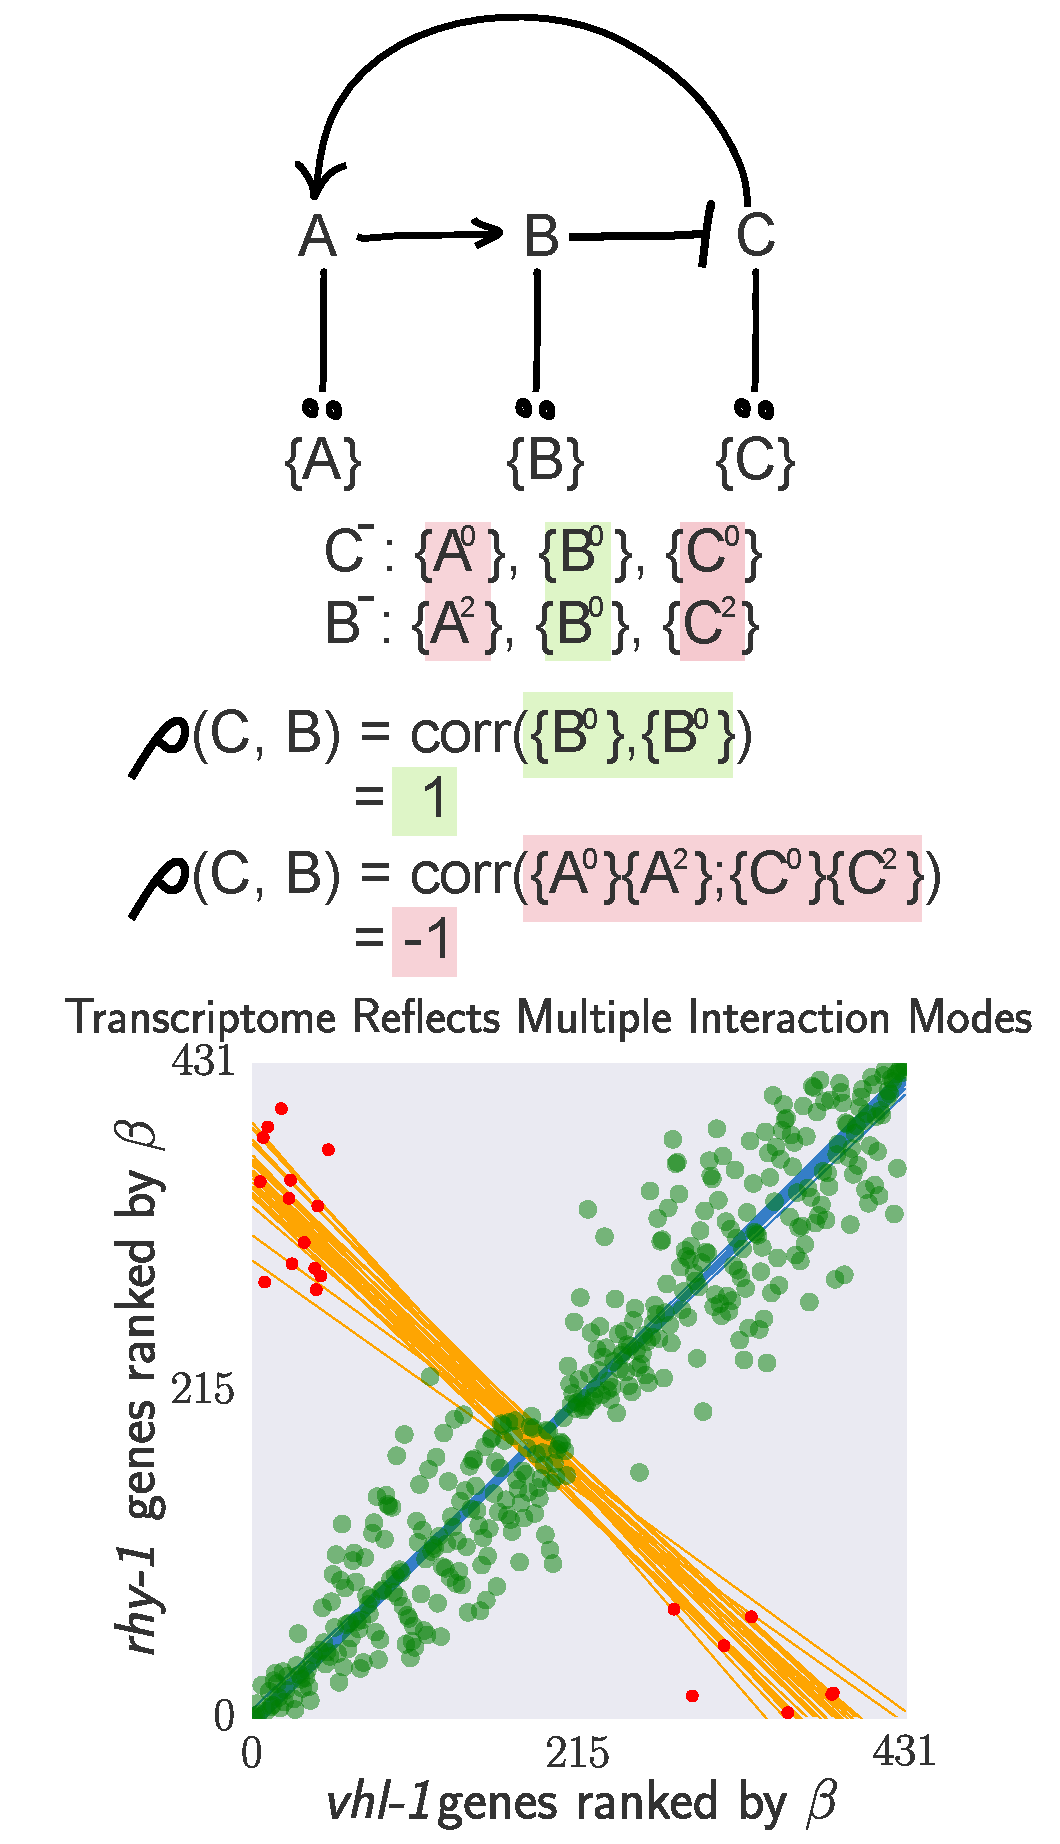
\includegraphics[width=\linewidth]{figs/correlative_genetics2.pdf}
\caption{
\textbf{Top}: A feedback loop can generate transcriptomes that are both
correlated and anti-correlated. \textbf{Bottom}: \hif{} transcriptome correlated
to the \rhy{} transcriptome. Green large points are inliers to the first
regression. Red small points are outliers to the first regression. Only the red
small points were used for the secondary regression. Blue lines are representative
samples of the primary bootstrapped regression lines. Orange lines are
representative samples of the secondary bootstrapped regression lines.
}
\label{fig:xpattern}
\end{figure}

If the logic above is correct, then it should be possible to decouple
transcriptomes in a logically consistent way. Currently, transcriptomes are
decoupled via subtractive logic. In other words, to identify the \rhy{}-specific
transcriptome (the effects of \rhy{} not dependent on \egl{}), subtractive logic
might suggest to find the overlap between the two transcriptomes. The genes that
are differentially expressed but are not in the overlap would then be considered
\rhy{}-specific transcriptomes. Such a gene set would consider of almost
700 genes. However, this approach suffers from a number of
drawbacks, principally that it does not take into account the relationship
between the two genes in question. Moreover, these genes have no testable properties:
i.e., a gene might not be in the overlap because it was not identified due to
chance in one of the two transcriptomes. In aggreggate, there is no pattern that
is present in these genes that can be used to identify them beyond overlapping
the two transcriptomes.

\rhy{} and \egl{} share a well-defined relationship. \rhy{} inhibits \cysl{},
which in turn inhibits \egl{}~\cite{Ma2012}. Therefore, loss of \rhy{} leads
to inactivation of \egl{}, which leads to increase in the cellular levels of
\hifp{}. \hifp{} in turn causes the mRNA levels of \rhy{} and \egl{} to increase,
as they are involved in the \hif{}-dependent hypoxia response. However, since
\rhy{} has been mutated, the observed transcriptome is \rhy{} null; \egl{} null;
\hifp{} on. The situation is similar for a knockout of \egl{}, except that \rhy{}
is not inactive, and therefore the observed transcriptome is the result of
\rhyp{} up; \egl{} null; and \hifp{} on. From this pattern, we conclude that
the \egl{} and \rhy{} transcriptomes should exhibit a cross-pattern: The positive
arm of the cross is the result of the \egl{} null; \hifp{} on dynamics; and the
negative arm reflects the different direction of \rhyp{} activity between
transcriptomes. However, no negative arm is visible (with the exception of two
outliers, which are annotated as pseudogenes in WormBase). Therefore, it is likely
that a large portion of all the transcriptomic effects of \rhyp{} in this dataset
are downstream of \egl{}.

Next, we wanted to know whether our dataset was able to capture \egl{}
\hif{}-independent transcriptomic effects. We have observed that deletion of
\hif{} leads to a modest increase in the transcription of \rhy{}, from which we
concluded that \eglp{} would be more active in the \hif{} mutant than in the
wild-type. Therefore, we searched for genes that were regulated in opposite
manner between the \hif{} and \hif{};\egl{} mutants, and that were regulated
in the same direction between the \hif{};\egl{} and \egl{} (or \rhy{}) mutants.
We were only able to find a single gene, \emph{clec-88}, which was down-regulated
in \hif{} mutants, but upregulated in every other mutant we studied. Although
it may be the case that \egl{} does not have a \hif{}-independent transcriptomic
phenotype, it is also possible that the change in \hifp{} dosage between a
wild-type normoxic animal and a \hif{} mutant is not sufficient to alter the
activity of \eglp{} to a consistently detectable level given our read-depth.
% Due
% to the privileged role of \eglp{} in controlling this circuit, the comparison
% between \hif{} and \egl{};\hif{} animals is the most important comparison for
% identifying an \egl{}-specific transcriptome.

We leveraged this genetic logic to identify a main hypoxia
response induced by removing inhibition on \hif{} (260 genes). Although the
hypoxic response is likely to involve between five and ten times more genes,
this is a conservative estimate that minimizes false negative results, since
these changes were identified in four independent genotypes with three replicates
each. We also identified a \vhl{}-specific response, resulting in \vhltargets{}
genes. We searched for candidates directly regulated by \hif{}.
Initially, we generated this list using the most stringent pattern
matching, but this revealed only 2 genes (\emph{R08E5.3} and
\emph{nit-1}). A relaxed set of conditions (target genes should go up in all
mutants that induce \hifp{}, and should not be up in \hif{} mutants) identified
\hiftargets{} candidate genes.

\subsubsection*{Enrichment analysis of the hypoxia response}
\label{sub:ea_hypoxia}
In order to validate that our transcriptomes were correct, and to understand how
functionalities may vary between them, we subjected each decoupled response to
enrichment analysis using the WormBase Enrichment
Suite~\cite{Angeles-Albores2016}.

\begin{figure}[tbhp]
\centering
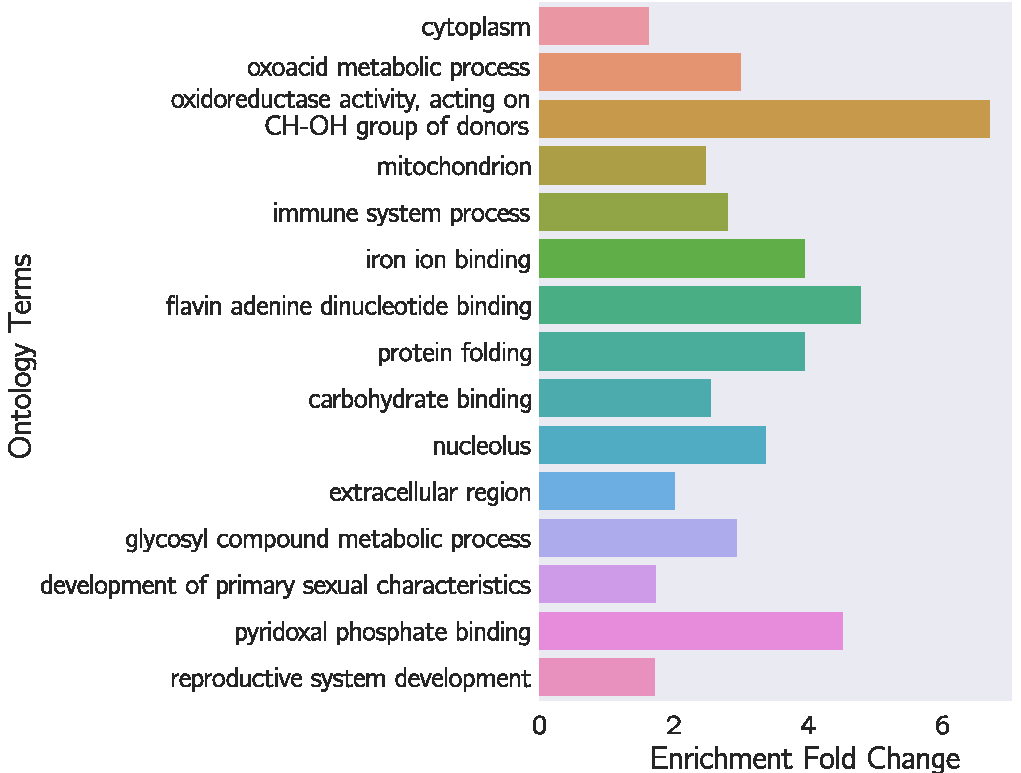
\includegraphics[width=\linewidth]{figs/hypoxia_response_gea.pdf}
\caption{
GEA of genes associated with the main hypoxia response. A number of terms
reflecting catabolism and bioenergetics are enriched.
}
\label{fig:hyp_gea}
\end{figure}

Gene enrichment analysis (GEA) showed that the terms `oxoacid metabolic process'
(\qval{3}, 3.4 fold-change, 19 genes),
`iron ion binding' (\qval{3}, 5.5 fold-change, 10 genes),
and `immune system process' (\qval{3}, 3.4 fold-change, 17 genes) were enriched
with the lowest q-values. GEA also showed enrichment of terms including
`electron carrier activity' (\qval{1}, 4.8 fold-change, 5 genes),
`mitochondrion' (\qval{2}, 2.5 fold-change, 20 genes)
and `respiratory chain' (\qval{1}, 4.6 fold-change, 4 genes) (see
Fig.~\ref{fig:hyp_gea}). Indeed, \hif{} has been implicated in
all of these biological and molecular functions~\cite{Luhachack2012,Ackerman2012,
Romney2011,Semenza2011}. Phenotype Enrichment Analysis (PEA) revealed that this
gene list was enriched in two phenotypes: `oxygen response variant' (\qval{2},
5.8 fold-change, 7 genes) and `pleiotropic defects severe early embryo' (\qval{2},
4.4 fold-change, 9 genes). The overrepresented terms from PEA and GEA are biologically
directly connected to the process we are studying, which suggests that we have
correctly identified the main hypoxic response. As a final test to guarantee the
quality of our data, we selected a set of 21 known reporters from the literature
and asked whether these reporters were present in our list. We found $5/21$ known
reporters, which constitutes a statistically significant result ($p<10^{5}$).
The small number of reporters found in this list probably reflects the conservative
nature of our estimates. We also analyzed the list of predicted \hif{} direct targets.
Phenotype Enrichment Analysis revealed that this list was significantly enriched in
`oxygen response variant' (\qval{2}, 12.3 fold-change, 4 genes) and Tissue Enrichment
Analysis (TEA) showed enrichment of the `coelomic system' (\qval{1}, 2.7 fold-change,
16 genes). The \vhl{}, \hif{}-independent specific transcriptome was also submitted
for enrichment analysis but no terms were significantly enriched.\todo{closer is missing.}

\subsection{Identification of non-classical epistatic interactions}
\label{sub:hifoh}
\hif{} has traditionally been viewed as existing in a genetic OFF state under
normoxic conditions. However, our dataset indicates that \hifn{} genes show
altered expression when it is removed in normoxic conditions. Moreover, we
observed positive genome-wide expression correlations between \hif{} expression
levels and \egl{}, \vhl{} and \rhy{} expression levels in spite of the negative
regulatory relationships between these genes and \hif{}. Such positive
relationships could indicate a different relationship between these genes
than has previously been reported. We wanted to explore whether these genome-wide
positive correlations were substantiated by epistatic analyses.

To perform epistatic analyses, we first identified genes that exhibited violations
of the canonical genetic model of the hypoxia pathway. To this end, we searched for
genes that exhibited different behaviors between the \egl{} and the \vhl{}
mutants, or between the \rhy{} and \vhl{} (we assume that all results from the
\rhy{} transcriptome reflect a complete loss of \egl{} activity). We found
\hifohtargets{} that satisfied this condition (see Fig.~\ref{fig:hif1oh}).
Additionally, many of these genes exhibited new kinds of epistasis. Namely,
\egl{} was epistatic to \vhl{}. Identification of a set of genes that have a
consistent set of relationships with between themselves suggests that we have
identified a new aspect of the hypoxia pathway.

\begin{figure}[tbhp]
\centering
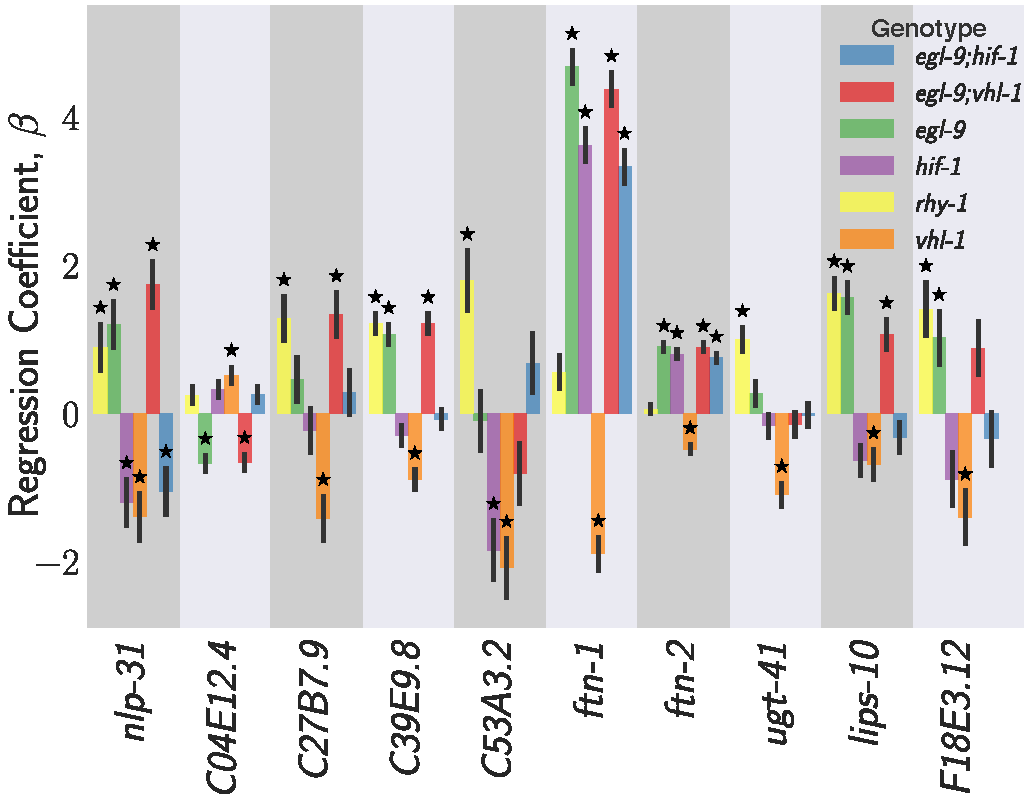
\includegraphics[width=\linewidth]{figs/hif1oh_epistasis.pdf}
\caption{
Genes that have altered differential expression between \egl{} and \vhl{} also
often exhibit the same epistatic patterns between \egl{} and \hif{}, and \egl{}
and \vhl{}, which suggests they are the result of the same biological effect.
}
\label{fig:hif1oh}
\end{figure}

In particular, we focused on three genes, \nlp{}, \ftna{} and \ftnb{}, which
epistasis patterns that we felt reflected the population well. As a sanity check,
we reviewed the literature, and found that \ftna{} and \ftnb{} are both described
in the literature as genes that are responsive to mutations in the hypoxia pathway.
Moreover, these genes have been previously described to have aberrant behaviors
previously~\cite{Ackerman2012,Romney2011}, specifically documenting the opposite
effects of \egl{} and \vhl{}. Probably as a reflection of the oddity of these
results, these studies showed that loss of \vhl{} suppresses \ftna{} and \ftnb{}
using both RNAi and alleles, which allays concerns of strain-specific interference.
Moreover, one of these studies showed that \vhl{};\hif{}
is epistatic to \hif{}~\cite{Ackerman2012}, and that loss of \hif{} is associated
with increased expression of \ftna{} and \ftnb{}. We observe that \hif{} is
epistatic to \egl{};\hif{}, and that \egl{} and \hif{} promote \ftna{} and
\ftnb{}
expression.\todo[inline]{see Romney2011 figure 2b; Ackerman2012 Fig. 3; Fig.6}
This further validates the quality of our RNA-seq data and the analysis, and
highlights the power of RNA-seq to identify novel interactions.

A qualitative epistatic analysis of \ftna{} and \ftnb{} reveals that \egl{} is
epistatic to \hif{}; that \vhl{} has opposite effects to \egl{}; and \vhl{} is
epistatic to \egl{}. Epistatic analysis of \nlp{} reveals similar relationships.
\nlp{} expression is decreased by loss of \hif{}, and promoted by \egl{}. However,
\egl{} is epistatic to \hif{}. Like \ftna{} and \ftnb{}, \vhl{} has the opposite
effect to \egl{}, but is also epistatic to \egl{}.

\subsection{Genome-wide effects of \hif{}}
\label{sub:metabolism}

\todo{This section is missing figures.}
The high quality of this dataset also provides us directly with a high-level
overview of the transcriptional responses that lead to physiologic and metabolic
changes in hypoxia. We wanted to better understand the transcriptional changes
associated with bioenergetic pathways in \cel{}. To this end, we extracted from
WormBase all genes associated with the tricarboxylic acid (TCA) cycle, the
electron transport chain (ETC) and with the \cel{} energy reserve (glycogen
metabolism, fatty acid metabolism, etc\ldots). Previous research has described
the effects of mitochondrial dysfunction in eliciting the hypoxia
response~\cite{Lee2010}, but transcriptional feedback from \hif{} into
bioenergetic pathways has not been well described in \cel{}, although it has been
extensively described in other organisms (see, for example~\cite{Semenza1994,
Semenza2012}).
\todo[inline]{I have searched the literature fairly thoroughly, and haven't
seen a complete transcriptional description of hif-1 induced changes in the TCA,
ETC.\@ Can anyone let me know if I missed something?}

\subsubsection{Bio-energetic pathways}

\todo[inline]{Bio-energetic or bioenergetic?}
Our data shows that most of the enzymes involved in the TCA cycle and in the ETC
are down-regulated when \hifp{} is induced in agreement with the previous
literature~\cite{Semenza2012}.\todo[inline]{Missing ETC citation} However,
\gene{fum-1} and the mitochondrial complex II stood out as notable exceptions to
the trend, as they were up-regulated in every single genotype that causes
deployment of the hypoxia response. \gene{fum-1} catalyses the reaction of
fumarate into malate, and complex II catalyses the reaction of succinate into
fumarate. Complex II has been identified as a source of reserve respiratory capacity
in neonatal rat cardiomyocytes previously~\cite{Pfleger2015}.\todo[inline]{Missing
discussion of why this is biologically relevant. Fumarate is a poison for egl-9.}
We found two energy reserve genes that were down-regulated by \hifp{}. \gene{aagr-1}
and \gene{aagr-2}, which are predicted to function in glycogen
catabolism~\cite{Sikora2010} were both down-regulated in all the relevant mutants.
Three distinct genes involved in energy reserve were up-regulated. These genes were
\gene{ogt-1}, an O-linled GlcNac Transferase; \gene{T04A8.7}, an ortholog of human
glucosidase acid beta (GBA); and \gene{T22F3.3}, an ortholog of human glycogen
phosphorylase isozymes.

\subsubsection{Protein synthesis and degradation}

\hif{} is also known to inhibit protein synthesis and translation in varied ways.
For example, \hif{} is known to control the translational machinery indirectly
via inhibition of mTOR~\cite{Brugarolas2004}. However, most reported effects of
\hif{} on the translation machinery are posttranslational, and no reports to date
show decreases in transcription of the ribosomal machinery in \cel{}. We used
the WormBase Enrichment Suite Gene Ontology dictionary~\cite{} to extract 143 genes
annotated as `structural constituents of the ribosome' and we queried whether they
were differentially expressed in our mutants. \egl{}, \vhl{}, \rhy{} and
\egl{};\vhl{} mutants showed differential expression of 91 distinct ribosomal
constituents (not all constituents were detected in all genotypes). For every one
of these genotypes, these genes were always down-regulated. In contrast, the
\hif{} mutant showed up-regulation of a single ribosomal constituent.

Next, we wanted to know whether \hif{} has any transcriptional effects on the
proteasomal constituents, because no such effects of \hif{} on the proteasome
have been reported in \cel{}. Out of 40 WormBase annotated proteasomal constituents,
we found 31 constituents that were differentially expressed in at least one of the
four genotypes that induce a hypoxic response. Every gene we found was down-regulated
in at least two out of the four genotypes we studied, although in each case the
down-regulation was minor. It is impossible to distinguish whether these animals
exhibit a decrease in proteasome expression is due to a lower requirement for
degradation in these animals due to constitutively depressed translation rates or
whether the decrease in expression is a direct result of \hifp{} stabilization.

% Previous studies have suggested that proteotoxicity from misfolded proteins is a
% major player in hypoxic induced death~\cite{Mehta2009,Fawcett2015}. One way to
% prevent proteotoxicity is to increase chaperone levels to allow unfolded clients
% to be refolded. We explored this possibility by extracting all 97 genes annotated
% in WormBase with the GO term `protein folding'. 44 genes were differentially expressed
% in \egl{}, \rhy{}, \vhl{} or \egl{};\vhl{} mutants. The majority of these
% genes were down-regulated. Down-regulated genes


\section*{Discussion}
\subsection*{The \cel{} hypoxia pathway can be reconstructed entirely from
             RNA-seq data}
We have presented the first genetic pathway reconstruction in a multicellular
organism using whole-organism RNA-seq to measure transcriptomic phenotypes.
We were able to reconstruct first-order and second-order interactions. We
were able to infer order of action (\rhy{} activates \egl{}, \egl{} and
\vhl{} inhibit \hif{}), and we were able to infer from genome-wide epistatic
measurements that \egl{} exerts \vhl{}-dependent and independent inhibition on
\hif{}.

In addition to reconstructing the pathway, our dataset afforded us the opportunity
to observe a wide variety of physiologic changes that occur when the \hif{}-dependent
hypoxia response is activated. In particular, we observed down-regulation of most
components of the TCA cycle and the mitochondrial electron transport chain.
As an exception, \gene{fum-1} and the mitochondrial complex II, which are involved
in fumarate metabolism within these pathways were up-regulated. The mitochondrial
complex II catalyses the reaction of succinate into fumarate. Complex II is known
to be important for hypoxic survival in rat cardiomyocyte cells~\cite{Pfleger2015}.
Complex II may play a similar role in \cel{}. The product of complex II
activity is fumarate. In mouse embryonic fibroblasts, fumarate has been
shown to antagonize \hifp{} prolyl hydroxylase domain (PHD) enzymes, which are
orthologs of \egl{}. Upregulation of complex II by \hifp{} during hypoxia may
therefore result in increased intracellular levels of fumarate, which in turn could
lead to artificially high levels of \hif{} (if the inhibitory role of fumarate is
conserved in \cel{}) even after hypoxic conditions have vanished in the absence
of concurrent metabolic changes.

Under this framework, the up-regulation of \gene{fum-1} agrees with intuition. By
up-regulating \gene{fum-1}, we speculate that \cel{} may be capable of harnessing
reserve respiratory capacity via complex II, while rapidly degrading the excess
fumarate that is generated. Degrading fumarate rapidly may allow \cel{} to
maintain plasticity in the hypoxia pathway, keeping the pathway sensitive to
oxygen levels.

\subsection*{Non-classical epistasis in the hypoxia pathway}
The observation of almost 30 genes that exhibit a specific pattern of non-classical
epistasis reveals new aspects of the pathway. Some of these non-classical
epistases had been observed previously, but no satisfactory mechanism has been
proposed to explain this biology. \citep{Romney2011} and \citep{Ackerman2012}
suggest that \hif{} integrates information on iron concentration in the
cell to bind to the \ftna{} promoter, but could not definitively establish
a mechanism.
In particular, it is unclear why deletion of \hif{} induces \ftna{}
expression, but deletion of \egl{} also causes induction of \ftna{} expression,
whereas \vhl{} removes this inhibition. Moreover, \citep{Luhachack2012} have
previously reported that certain genes important for the \cel{} immune response
against pathogens reflect similar expression patterns. Their interpretation
was that \gene{swan-1}, a binding partner to \egl{}~\cite{Shao2010}, is important
for modulating \hifp{} activity somehow. The lack of a conclusive double
mutant analysis in this work means the role of \gene{swan-1} in modulation of
\hifp{} activity remains to be demonstrated.
At any rate, mechanisms that call for additional
transcriptional modulators become more unlikely given our data the large number of
genes with different biological functions that exhibit the same pattern.

\begin{figure}[tbhp]
\centering
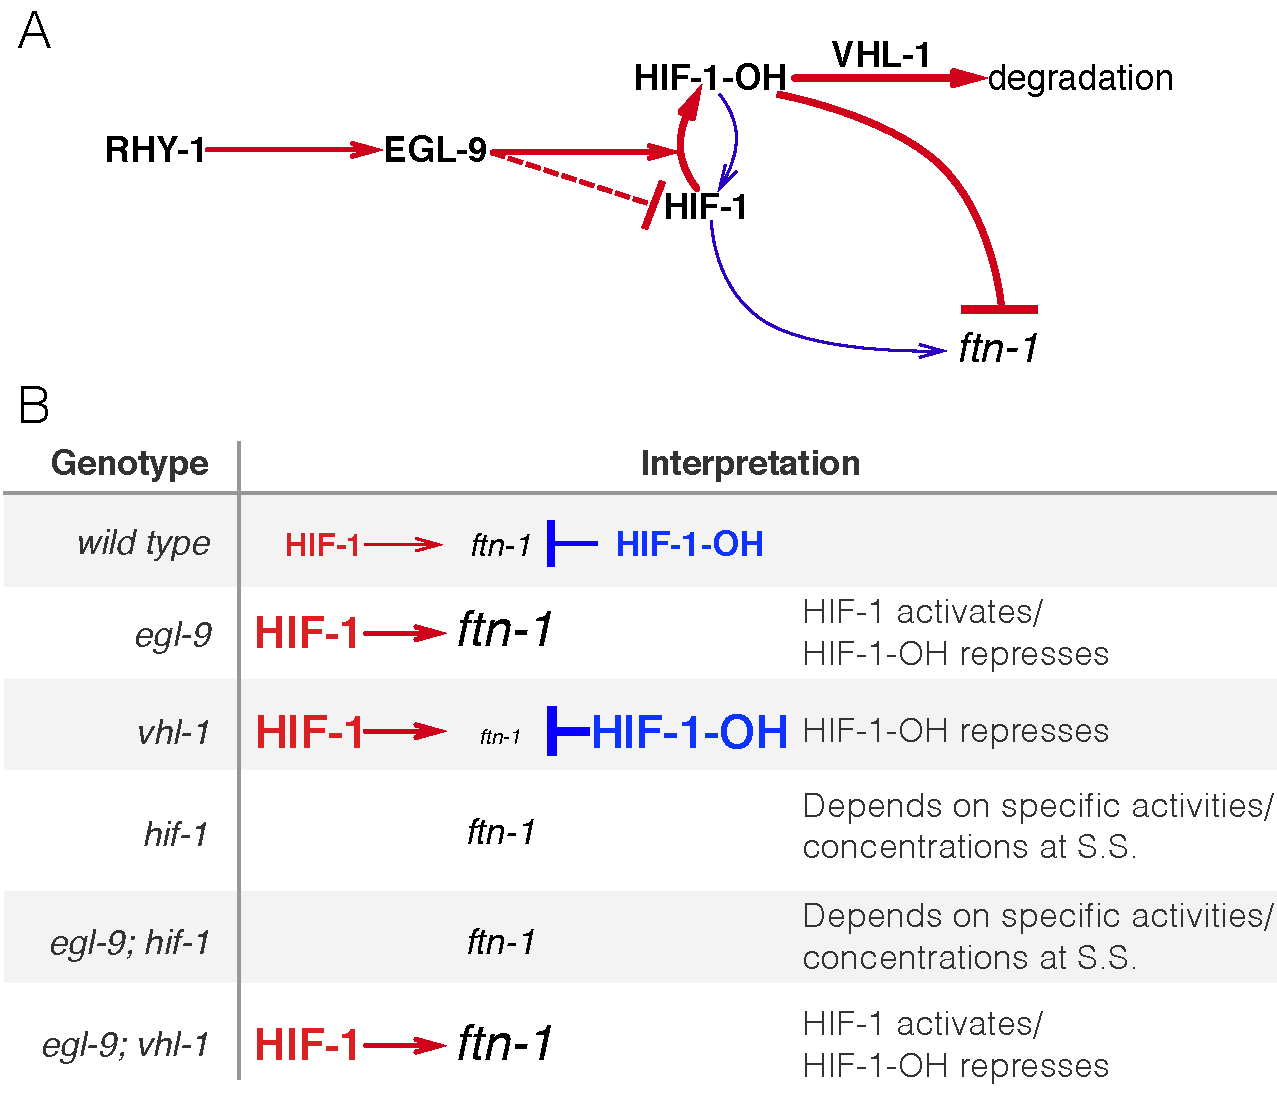
\includegraphics[width=\linewidth]{figs/hif1oh_model.pdf}
\caption{
A toy model showing that an interpretation where \hifp{}-hydroxyl
is biochemically active can potentially explain how genes that exhibit
non-canonical epistasis are regulated.
}
\label{fig:hif1oh_table}
\end{figure}


One way to resolve this problem without invoking additional genes is to
model \hifp{} as a protein with both activating and inhibiting states. In fact,
\hifp{} already exists in two states in \cel{}: unmodified \hifp{} and
\hifp{}-hydroxyl. Under this model, \hifp{}-hydroxyl would inhibit gene expression,
whereas \hifp{} drives it. \vhl{} stabilizes \hifp{}-hydroxyl, which will
cause inhibition of genes to which both forms of the protein bind; whereas \egl{}
selectively removes all \hifp{}-hydroxyl, indirectly stimulating accumulation of
\hifp{} and promoting gene activity. Whether deletion of \hif{} is activating or
inhibiting will depend on the relative contributions of each protein activity
under normoxia (see Fig.~\ref{fig:hif1oh_table}).

The possibility that \hifp{}-hydroxyl has a function has not been previously
considered in the existing literature, although experts have wondered about
the possibility that \hifp{}-hydroxyl may have transcriptional effects independent
of \hifp{} (William Kaelin, pers.\ comm.). Here, we draw multiple, varied lines
of circumstantial evidence to suggest that \hifp{} hydroxylation plays a role
in the functionality of the hypoxia pathway. First, \hifp{}-hydroxyl is
challenging to study genetically because no mimetic mutations are available with
which to study the pure hydroxylated \hifp{} species. Moreover, mutations in
the Von-Hippel Landau gene stabilize the hydroxyl species, but also increase the
quantity of \hifp{} by mass action. Since \hif{} exists at low levels in cells
under normoxic conditions, total \hifp{} protein (unmodified \hifp{} plus
\hifp{}-hydroxyl) is often tacitly assumed to be vanishingly rare.

Our data shows that there are hundreds of genes that change expression in response
to loss of \hif{} under normoxic conditions. This establishes that there is sufficient
total \hifp{} protein to be biologically active. Previous literature showing
substantial changes in mRNA expression of \ftna{} support our claim that under
normoxia \hif{} is biologically relevant. Moreover, our analysis of the
hypoxia pathway using transcriptomic phenotypes reveals that \hif{} shares main
positive correlations with \egl{}, \rhy{} and \vhl{}, and that each of these genes
also shows a set of genes negative rank-ordered expression correlations. These
cross-patterns between all controllers of \hif{} and \hif{} can be most easily
explained if \hifp{}-hydroxyl is biologically active.

An additional argument in favor of the activity of \hifp{}-hydroxyl is a
homeostatic argument. At any point in time, the cell must measure the levels of
multiple small molecules at once. Strictly speaking, the \hif{}-dependent hypoxia
response integrates information from O$_2$, $\alpha$-ketoglutarate
(2-oxoglutarate) and iron concentrations in the cell. One way to encode this
information is by encoding it only in the effective hydroxylation rate of \hifp{} by
\eglp{}. Then the dynamics in this system will evolve exclusively as a result of
the total amount of \hifp{} in the cell. Such a system can be sensitive to
fluctuations in the absolute concentration of \hifp{}~\cite{Goentoro2009a}. In the
case of severe hypoxia, when the levels of \hifp{} are expected to rise enormously
within the cell, simple information integration via \egl{} would probably be
sufficient encoding for a subset of protective genes.

For yet other set of genes that must change expression in response to the hypoxia
pathway, it may not make as much sense to integrate metabolite information
exclusively via \eglp{}-dependent hydroxylation of \hifp{}. In particular, genes
that may increase survival in mild hypoxia may benefit from homeostatic regulation
that is not susceptible to transient changes in protein copy number. Likewise,
genes that are involved in iron or $\alpha$-ketoglutarate metabolism
(such as \ftna{}) may benefit from being able to sense, accurately, small and
consistent deviations from basal concentrations of these metabolites. For these
genes, the information may be better encoded by using \hifp{} and
\hifp{}-hydroxyl as an activator/repressor pair. Such paradoxical circuits are
known to possess distinct advantages for controlling output in a manner that
is robust to transient fluctuations in the levels of their
components~\cite{Hart2012,Hart2013}.

Our RNA-seq data suggests that one of the targets that \hif{} may target
paradoxically is \rhy{}. Although \rhy{} does not exhibit non-classical epistasis,
genotypes that included a loss-of-function \hif{} caused increased \rhy{} activity.
We speculate that if \rhy{} is controlled by both \hifp{} and \hifp{}-hydroxyl,
then this might mean that \hif{} regulates the expression of its pathway (and
therefore itself) in a manner that is robust to total \hifp{} levels.

\subsection{Looking forward}
We have demonstrated the first complete reconstruction of a genetic pathway using
whole-organism RNA-seq in a complex multicellular organism. Future work must
rigorously demonstrate that macroscopically derived genetic rules of interaction
hold genome-wide, and if not, how genetic rules deviate from expectations.


\matmethods{
\label{methods}
\subsection*{Nematode strains and culture}
Strains used were N2 wild-type Bristol, CB5602 \vhl{}(ok161), CB6088
\egl{}(sa307) \hif{}(ia4), CB6116 \egl{}(sa307) \vhl{}(ok161), JT307
\egl{}(sa307), ZG31 \hif{}(ia4), RB1297 \rhy{}(ok1402).
ZG31\hif{}(ia4) is a null mutant of \hif{} which deletes 1231 bp of the second,
third and fourth exons.
JT307 contains the null mutant \egl{}(sa307) which is a  243 bp deletion.
RB1297 contains null mutation \rhy{}(ok1402) with an estimated 700 bp deletion
constructed by the OMRF Knockout Group. CB5602 contains the deletion mutation of
\vhl{}(ok161).
CB6088 contains \egl{}(sa307);\hif{}(ia4). % and was constructed by J.~Hodgkin.
CB6116 contains \egl{}(sa307) \vhl{}(ok161). % and was constructed by J.~Hodgkin.
All strains were provided by the CGC, which is funded by NIH Office of Research
Infrastructure Programs (P40 OD010440).  All lines were grown on standard
nematode growth media (NGM) plates with seeded with OP50 \ecol{} at 20\degree{}C
(Brenner 1974).

\subsection*{RNA Isolation}
Unsynchronized lines were grown on NGM plates at 20C and eggs harvested by
sodium hypochlorite treatment. Eggs were plated on 6 to 9 small 5cm NGM plates
with ample OP50 \ecol{} at a density chosen to avoid starvation and grown at
20\degree{}C.  Worms were staged and harvested based on the time after plating,
vulva morphology and the absence of eggs.  Approximately 30--50 non-gravid young
adults (YA) were picked and placed in 100$\mu$L of TE pH 8.0 at 4\degree{}C in
$0.2$mL PCR tubes.   After settling and a brief spin in microfuge approximately
$80\mu$L of TE was removed from the top of the sample and individual replicates
were snap frozen in liquid N2. These replicate samples were then digested with
Proteinase K for 15min at 60\degree{} in the presence of 1\% SDS and 1.25$\mu$L
RNA Secure (Ambion AM 7005). RNA samples were then taken up in 5 Volumes of
Trizol (Tri Reagent Zymo Research) and processed and treated with DNAase I using
Zymo MicroPrep RNA Kit (Zymo Research Quick-RNA MicroPrep  R1050).
RNA was eluted in dH2O and divided into aliquots and stored at -80\degree{}C.
One aliquot of each replicate was analyzed by both NanoDrop for impurities,
Qubit for concentration and then analyzed on an Agilent 2100 BioAnalyzer.
Replicates were selected that had RNA integrity numbers (RIN) equal or greater
than 9.0 and showed no evidence of bacterial ribosomal bands, except for the
ZG31 mutant where one of three replicates had a RIN of 8.3.

\subsection*{Library Preparation and Sequencing}
Libraries were sequenced on Illumina HiSeq2500 in single read mode with the read
length of 50 nt to an average depth of 15 million reads per sample following
manufacturer's instructions. Base calls were performed with RTA 1.13.48.0
followed by conversion to FASTQ with bcl2fastq 1.8.4.

\subsection*{Read Alignment and Differential Expression Analysis}
We used Kallisto to perform read pseudo-alignment and performed differential
analysis using Sleuth. We fit a generalized linear model for a transcript $t$ in
sample $i$:

\begin{equation}
  y_{t,i} = \beta_{t, 0} + \beta_{t, genotype}\cdot{}X_{t, i} +
  \beta_{t, batch}\cdot{}Y_{t, i} + \epsilon_{t, i}
\end{equation}

where $y_{t, i}$ are the logarithm transformed counts; $\beta_{t, genotype}$ and
$\beta_{t, batch}$ are parameters of the model, and which can be interpreted as
biased estimators of the log-fold change; $X_{t, i}, Y_{t, i}$ are indicator
variables describing the conditions of the sample; and $\epsilon_{t, i}$ is the
noise associated with a particular measurement.

\subsection*{Genetic Analysis}
Genetic analysis of the processed data was performed in Python 3.5. Our scripts
made extensive use of the Pandas, Matplotlib, Scipy, Seaborn, Sklearn, Networkx,
Bokeh, PyMC3, and TEA libraries~\cite{Team2014,McKinney2011,Oliphant2007,
Pedregosa2012,Salvatier2015,VanDerWalt2011,Hunter2007,Angeles-Albores2016,Waskom}.
Our analysis is available in a Jupyter Notebook~\cite{Perez2007}. All code and
required data (except the raw reads) are available at
\url{https://github.com/WormLabCaltech/mprsq} along with version-control
information. Our Jupyter Notebook and interactive graphs for this project can be
found at \url{https://wormlabcaltech.github.io/mprsq/}. Raw reads were deposited
at XXXXXXXXXXX
}

\showmatmethods{}% Display the Materials and Methods section

\acknow{
This work was supported by HHMI with whom PWS is an investigator
and by the Millard and Muriel Jacobs Genetics and Genomics Laboratory at
California Institute of Technology.
This article was written with support of the Howard Hughes Medical Institute.
We thank Hillel Schwartz for his help in the fun analysis of ftn-1 epistasis.
We would like to thank Jonathan Liu, Han Wang, and Porfirio Quintero for helpful
discussion.
}

\showacknow{} % Display the acknowledgments section

% \pnasbreak splits and balances the columns before the references.
% If you see unexpected formatting errors, try commenting out this line
% as it can run into problems with floats and footnotes on the final page.
% \pnasbreak{}

% Bibliography
\bibliography{citations}

\end{document}
